\chapter{Person Detection Development}
\label{chapter3}

\section{Deep Learning Approach}

To develop the person detection module two different approaches were identified. The HOG algorithm and deep-learning based models. Both methods making use of the incoming RGB data from the on-board RGB-D sensor.

The Histogram of Oriented Gradients (HOG) and its possible variances such as the Oriented Histograms of Flow and Appearance (OHFA) and the AdaBoosted version was the first choice for the task, due to its simplicity in the integration as the method was already present in the OpenCV library. However, the method's performance was acceptable only in perfect conditions due to the mechanics of the algorithm, mainly when people are standing in up-right positions in sparse environments and with no or little occlusions. False positives were also another problem encountered as shown in the pictures below. Moreover, the sliding window technique used by the algorithms is rather inefficient as it has to search through the whole frame, making it computationally expensive for large frames.

On the other hand the deep-learning model proved to work really well under circumstances where HOG failed, such as when people are sat or not exactly standing, when they are facing with their back and with partial body occlusion or when only a section of the body is visible. Moreover, due to the mechanics of the algorithm each detection is accompanied with its probability of being a person, therefore allowing to discard detections with a low probability, something that was not possible if with HOG.

Therefore the SSD deep-learning model was chose over HOG.

\begin{figure}[H]
    \begin{subfigure}{.5\textwidth}
        \centering
        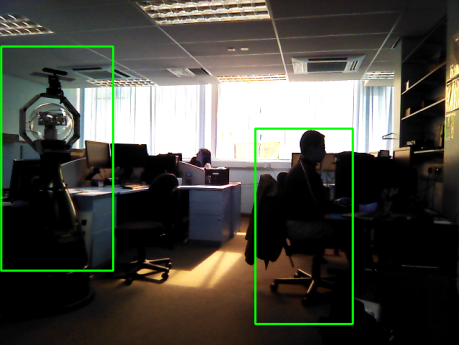
\includegraphics[width=.8\linewidth]{images/chapter3_hog.png}
        \caption{HOG detection with false positive.}
	\end{subfigure}
    \begin{subfigure}{.5\textwidth}
        \centering
        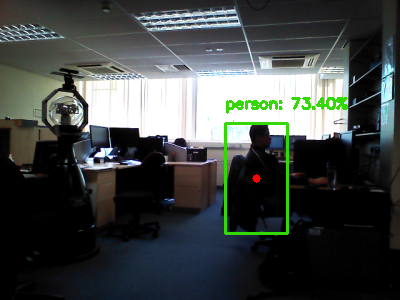
\includegraphics[width=.8\linewidth]{images/chapter3_dnn.png}
        \caption{SSD detection with no false positives.}
	\end{subfigure}
    \label{fig:hog}
\end{figure}

\subsection{Stack}

The stack used for the development of the detection module includes the Python programming language and the OpenCV library.

The choice to use Python derives from the nature of the project. In fact being it an \textbf{Exploratory Software} product there was a lot of prototyping phases to it before settling for particular approaches or methodologies, making of Python a natural choice for its dynamic behaviour and its ease of implementation. Moreover, both the ROS interfaces as well as the OpenCV library used offered Python bindings to call their relative APIs.

Version 3 of the Python programming language was been used in particular along with OpenCV 2.4.8 and 3.4.0 to relatively access Indigo's interfaced \textbf{CvBridge} modules and the \textbf{dnn}\footnote{deep-neural-network} module to work with the serialised SSD model.

Two different versions of OpenCV were used because the ROS indigo version used comes with de-facto static bindings for version 2.4.8 of the computer vision library. No easy install was available to upgrade to the latest version of OpenCV, required for the dnn module, which would still be compatible with Indigo's CvBridge module and a ROS distro upgrade wasn't an option given the need for the Indigo version for compatibility with TIAGo. The only remaining choice was to directly deal with a source installation and possibly fix the broken stating linkages along the way, which due to time constraints wasn't an option either. Virtual environments were instead used to solve issue.

\subsubsection{Virtual Environment Set-up}

A virtual environment is a cooperatively isolated runtime environment that allows Python users and applications to install and upgrade Python distribution packages without interfering with the behaviour of other Python applications running on the same system \cite{website:virtualEnv}.

To make use of such an environment some steps need to be taken. First of all the python package installer (pip) need to be installed if not already installed and upgraded to the latest version if any available. The last point is of particular importance as to access later on the latest version of OpenCV through pip, this has to be upgraded to the latest version as well.

The next step consists in installing the virtual-environment and the virtual-wrapper via pip which offers a higher level interface for the former to make the creation of the personalised environment easier. However, before proceeding to the actual creation of the environment the package installer cache needs to be cleaned in order to avoid conflicting issues with older versions present in the cache, which can be done with the following command:

\begin{lstlisting}[language=bash]
$ sudo rm -rf ~/.cache/pip
\end{lstlisting}

Next is the actual creation of the virtual-environment using the \textbf{mkvirtualenv} command made available through the virtual-wrapper package, that takes as a compulsory argument the name of environment, in this case harn, and as an optional one the Python version to be installed within it. In this particular circumstance Python3 was installed as it is a compulsory requirement for the OpenCV version to be installed. The install command is as follows:

\begin{lstlisting}[language=bash]
$ mkvirtualenv harn -p Python3
\end{lstlisting}

Finally the virtual-environment needs to be made accessible through simple bash commands so as to activate and de-activate the environment easily. For this, the created virtual environment is exported in the \textbf{.bashrc} file which makes it available to all future bash sessions upon start. The export command is as follows:

\begin{lstlisting}[language=bash]
$ export WORKON_HOME=$HOME/.virtualenvs
\end{lstlisting}

\subsubsection{OpenCV 3.3.0 Installation}

Once the environment is set-up, activating and de-activating it is as easy as a matter of calling the \textbf{workon} and \textbf{deactivate} commands, also made available by the virtual-wrapper package. Given that Python3 was already installed at the moment the virtual-environment was created, what remains is to only install the latest OpenCV version which including the needed dnn module within the environment. The following bash snippet shows the interaction with the environment and the installation process:

\begin{lstlisting}[language=bash]
$ workon harn # This activates the environment called harn
(harn)$ pip install opencv-contrib-python # Installs OpenCV 3.3.0
(harn)$ deactivate # This de-activates the environment
$ # Now the environment is not active anymore
\end{lstlisting}

Whenever the detection module needs to be executed this takes place in the isolated and activated harn virtual-environment where the latest OpenCV version and Python3 bindings are made available. The remaining modules are run in normal environments.

\clearpage

\subsection{Module design}

The final solution design was affected by the Indigo-OpenCV compatibility issue introduced in the before. More precisely, the detection module is not able to convert beforehand the RGB data incoming from the subscription into an OpenCV specific format, such as MAT, as the CvBridge interface is incompatible the latest version of OpenCV.

Hence the decision to split the single detection module into two different modules, with one component performing the conversion and the other the detection. The conversion module is accountable for the conversion of the raw image into a MAT format using the standard OpenCV 2.4.8 version and the compatible CvBridge interface. The detection module instead is solely responsible to perform the detection process on the converted image.

\subsection{OpenCV conversion}

The conversion module is implemented as a collection of routines in the \textbf{cv\_conversion.py} file made available in the deliverables. The steps to the conversion task are the following:

\begin{enumerate}
  \item Image topic subscription
  \item Callback conversion
  \item Conversion storage
\end{enumerate}

\subsubsection{Image Topic Subscription}

This step consists in subscribing to the raw stream of data made available by the robot's sensors, in particular the raw image data coming from the RGB-D sensor. However, before being able to realise the subscription a node has to be created. In fact, by making use of the ROS middle-ware, all communications happen over topics which allow the instances of the ROS graph, called nodes, to interact with each other by publishing or subscribing over the topic channels. 

To create the node the \textbf{rospy} library and its \textbf{init\_node} routine is used and whose arguments are two. The node's name so that is can be distinguished amongst the possible hundreds of nodes running in the graph, and a boolean flag, which if TRUE, adds random numbers to the node's name end to ensure its uniqueness \cite{website:nodes}. The following is the function call:

\begin{lstlisting}
rospy.init_node('cv_conversion', anonymous=True)
\end{lstlisting}

Once the node is created, the subscription is a matter of using the \textbf{Subscriber} routine available through the \textbf{rospy} library. The Subscriber method takes three arguments. The first one is the topic string where the raw RGB data are being published by the robotic system in use, in this case \textbf{xtion/rgb/image\_raw}. The second argument is message type being received through the subscription, ROS in fact offers many built-in messages type, but for this particular subscription the data received is a stadard\_msg/Image, which before being used has to be imported at the top of the script. The third and last argument is the callback function called once the data is received and whose task is to manipulate the raw information. The subscription call is as follows:

\begin{lstlisting}
rospy.Subscriber("/xtion/rgb/image_raw", Image, toMat)
\end{lstlisting}

\subsubsection{Callback Conversion}

The callback function has the task to manipulate the received data through the subscription. A callback function called \textbf{toMat} is defined which takes as argument the image\_raw data afterwards converted. However before describing the conversion step, it is interesting to note how the data is actually passed to the function. In fact, everything is handled by the Subscriber method which bundles the data and does the call to the function reference passed as an argument, hence no step in between is actually required.

The data conversion uses the \textbf{imgmsg\_to\_cv2} routine which is a method belonging to the CvBridge module. The function takes two arguments, the ROS image message to be converted and the encoding to convert it into. In this case these are the image\_raw passed to the callback function and bgr8. The conversion routine is as follows:

\begin{lstlisting}
cv_image = CvBridge().imgmsg_to_cv2(rgb_image, 'bgr8')
\end{lstlisting}

\subsubsection{Conversion storage}

Lastly the converted image has to be made available to the detection module for the detection process. This is exactly why the conversion was stored in a variable instance named \textbf{cv\_image}, as this is passed as a parameter to a second function whose task is just to save the image to the disk. A function called \textbf{store} is defined that takes as input the OpenCV image and calls the \textbf{imwrite} routine available through OpenCV to store the converted image in the specified path. The function call is as follows:

\begin{lstlisting}
cv2.imwrite(PATH + "/data/converted/image.png", cv_image)
\end{lstlisting}

where \textbf{PATH} is a constant variable storing a dynamic path to the folder used for the storage, so that no issues arise if the package is cloned in different paths by different user. The \textbf{path} python library is used to facilitate the path planning. The variable definition is as follows:

\begin{lstlisting}
PATH = str(Path(os.path.dirname(os.path.abspath(__file__))).parents[0])
\end{lstlisting}

\subsection{OpenCV detection}

The detection module, differently from the conversion component is implemented as a class in the \textbf{human\_detection.py} file made available in the deliverables. The steps to the detection process are the following:

\begin{enumerate}
  \item Model de-serialisation
  \item Image loading
  \item Feed-forward
  \item Process detections
  \item Message publication
\end{enumerate}

\subsubsection{Model De-Serialisation}

The original MobileNet version of the SSD model presented in the previous chapter was trained using Google's TensorFlow machine learning library by Howard et al. \cite{paper:MobileNets}. However, the version used for the project embedding makes use of the Caffe version trained by chuanqi305 \cite{website:chuanqi305}.

The trained model is able to detect over 20 different objects in images and is made available through serialised files that include the the \textbf{MobileNetSSD\_deploy.caffemodel} as well as the \textbf{MobileNetSSD\_deploy.prototxt}. The former defines the internal states and parameters for each layer, while the latter describes the architecture of network such as the input dimensions, the number of layers and the base network used as well as the activation function used.

Given that the neural network is serialised a de-serialisation process is requires. The dnn module introduced in version 3.3 of OpenCV is used to load the serialised Caffe model. Caffe trained networks are not the only accepted networks, as routine can work with a variety of other machine learning frameworks, including TensorFlow and Keras.

The de-serialisation or loading process does happen at the constructor level of the class that implements the detection module. In fact, by using the object-oriented-design a single instance can be used to handle all detection requests afterwards, therefore avoiding to load the network multiple times as only one de-serialisation is needed at the instantiation level. To perform the loading the \textbf{readFromCaffe} routine belonging to the dnn module's namespace is called, to which both the prototxt and .caffemodel files are passed as arguments as follows:

\begin{lstlisting}
self.net = cv2.dnn.readNetFromCaffe("prototxt.txt", "model.caffemodel")
\end{lstlisting}

\subsubsection{Image loading}

A further step is required before running the feed-forward routine made available through the de-serialisation of the model. This consists in actually loading the image to be fed to the neural network which was previously converted by the conversion module. OpenCV's \textbf{imread} routine is used for the task and whose main argument is the path to the image. The function call is as follows:

\begin{lstlisting}
cv_image = cv2.imread(self.path + "/data/converted/image.png")
\end{lstlisting}

\subsubsection{Feed-forward}

The feed-forward process consists in feeding the loaded image to the neural network, which runs the detection algorithm to find humans within the input image. However, before running the algorithm a couple more variables need to be initialised, as they are required by the algorithm. These are the target variable, that identifies the class category of interest to be detected, which in this case corresponds to the value 15 as people is the 15th category out of the 20 available, and the confidence variable which determines the minimum probability that a detection needs to have to be considered a good detection, in this case 0.5 turned out to be a good value. The array of targets containing all the possible categories is also defined.

Input wise, the network accepts multiple image colour spaces, including grayscale and RGB with the only constraint that the input dimensions are of 300x300 pixels. This means that the original input has to undertake a pre-processing step to scale it down to the required size. Moreover, mean-subtraction and scaling are also applied to the resized image via the \textbf{blobFromImage} function to further improve the chances of obtaining a correct detection \cite{website:blobFromImage}. The input preparation logic is as follows:

\begin{lstlisting}
# Resize image
resized = cv2.resize(frame, (300, 300))
# Apply pre-processing steps
blob = cv2.dnn.blobFromImage(resized, 0.007843, (300, 300), 127.5)
\end{lstlisting}

The rest of the detection process is straightforward as it is a matter of passing the pre-processed image to the network and run the feed-forward process. The dnn module offers routines for both of these tasks, by respectively calling the \cite{setInput} method on the previously network instance and passing it the blob object as shown below:

\begin{lstlisting}
self.net.setInput(blob)
\end{lstlisting}

Then the detections can be obtained by running the \textbf{forward} method on the same network instance as follows:

\begin{lstlisting}
detections = self.net.forwards()
\end{lstlisting}

\subsubsection{Process Detections}

The network is trained to recognise twenty different categories, however, this project is only interested in detecting people presence in the image, without much concern about any other object. Hence, within the iteration that loops over the detections returned by the feed-forward process, which is multi-dimensional array, a conditional statement is added that checks whether the detection ID is equal to our target variable defined previously. The confidence variable is also used within the same conditional statement to check that the person labelled detection is over a certain threshold by using an AND connective.

\begin{lstlisting}
# Loop over the detections
for i in np.arange(0, detections.shape[2]):
	# Get detection probability
	confidence = detections[0, 0, i, 2]

	# Get ID of the detection object
	idx = int(detections[0, 0, i, 1])

	# Filter out non-human detection with low confidence
	if confidence > self.confidence and idx == self.target:
    	# Rest of the logic goes in here
\end{lstlisting}

\textbf{Message publication}

Many are the information made available by the detections tensor, in fact, the confidence and the categorical class are just two of these. The other important detail used in the project is the actual position of the person in the RGB frame, which for each detection is in terms of its top-left and bottom-right point. Hence, the width, height and consequently the centre point of the bounding-box around the detected person can be easily computed.

The publisher-subscriber is the main ROS communication paradigm, where a node can publish over a particular topic different messages and subscribe to as many others. Therefore, to allow the rest of the package modules to interact with each other, the results from the feed-forward algorithms are made available over a topic called \textbf{detections}, that publishes a custom message defined for the project named \textbf{Detections}. The \textbf{Publisher} routine is used for this, which takes as the first argument the topic's name, followed by the message type and lastly the buffer size as follows:

\begin{lstlisting}
self.detection_pub = rospy.Publisher('detections', Detections, queue_size=5)
\end{lstlisting}

ROS already comes with standard data-types such as int, float and many others. Nonetheless, the creation of a new custom message to be used within a package is straightforward. First a \textbf{msg} folder is created at the root level of the package, which will hold the defined messages. Two messages are then created within the msg folder, one called \textbf{Detection.msg} which holds the details of the single detection, and another named \textbf{Detections.msg} that acts as a collection of all the details for all the detections that passed the if statement criteria. The two message definitions for the Detection.msg(left) and the Detections.msg(right) are shown below:

\begin{multicols}{2}
  \begin{itemize}
    \item int32 ID
    \item int32 centre\_x
    \item int32 centre\_y
  \end{itemize}

  \columnbreak

  \begin{itemize}
    \item Header header
    \item int32 number\_of\_detections
    \item Detection[] array
  \end{itemize}
\end{multicols}

The fields of the Detection message consist in an 32 bits integer value, that will serve in later modules to correspond which distance or pose is to which detection, another 32 bits integer values that stores the x-coordinate of the centre point of the detection and finally a 32 bits integers for the the y-coordinate of the centre point of the detection. Publishing each detection message by itself would not make sense, hence the need for the Detections message that has as fields a header storing information about the time-stamp of the creation, a 32 bits integer storing the number of the total detections for the input image and a collection of Detection messages pushed to the array. These message declaration before being available need to be added to the CMAKE file at the root of the package and built using \textbf{catkin build}.

For each positive detection in loop, a new Detection message instance is created and its fields are populated using Python's field access syntax. The ID takes the value of the current number of detections which at first is 0 and is increased at every loop iteration and set back to 0 at the end of the loop. The centre point of the detection's bounding-box is computed using the top-left and bottom-right information from the detections tensor for the specific detection, and its x and y coordinates are then stored in the relative fields. Every Detection message is then pushed to the Detections message array field using a simple append. The Detections message instance is a global one defined in the constructor, which get re-instantiated at the end of each loop. The population is as follows:

\begin{lstlisting}
# Create Detection message
detection = Detection()

# Populate Detection message
detection.ID = self.number_of_detections
detection.centre_x = centre_ratio_point[0]
detection.centre_y = centre_ratio_point[1]

# Push Detection message to Detections array field
self.detections.array.append(detection)
\end{lstlisting}

At the end of each feed-forward request, the Detections message instance is pushed to the detections topic, previously defined, using the \textbf{publish} method on the publisher instance, which takes as its only argument the message to be published, in this case self.detections as follows:

\begin{lstlisting}
self.detection_pub.publish(self.detections)
\end{lstlisting}

An example output of the detections topic using the \textbf{rostopic echo} command is shown below:

\begin{figure}[!htbp]
  \begin{center}
    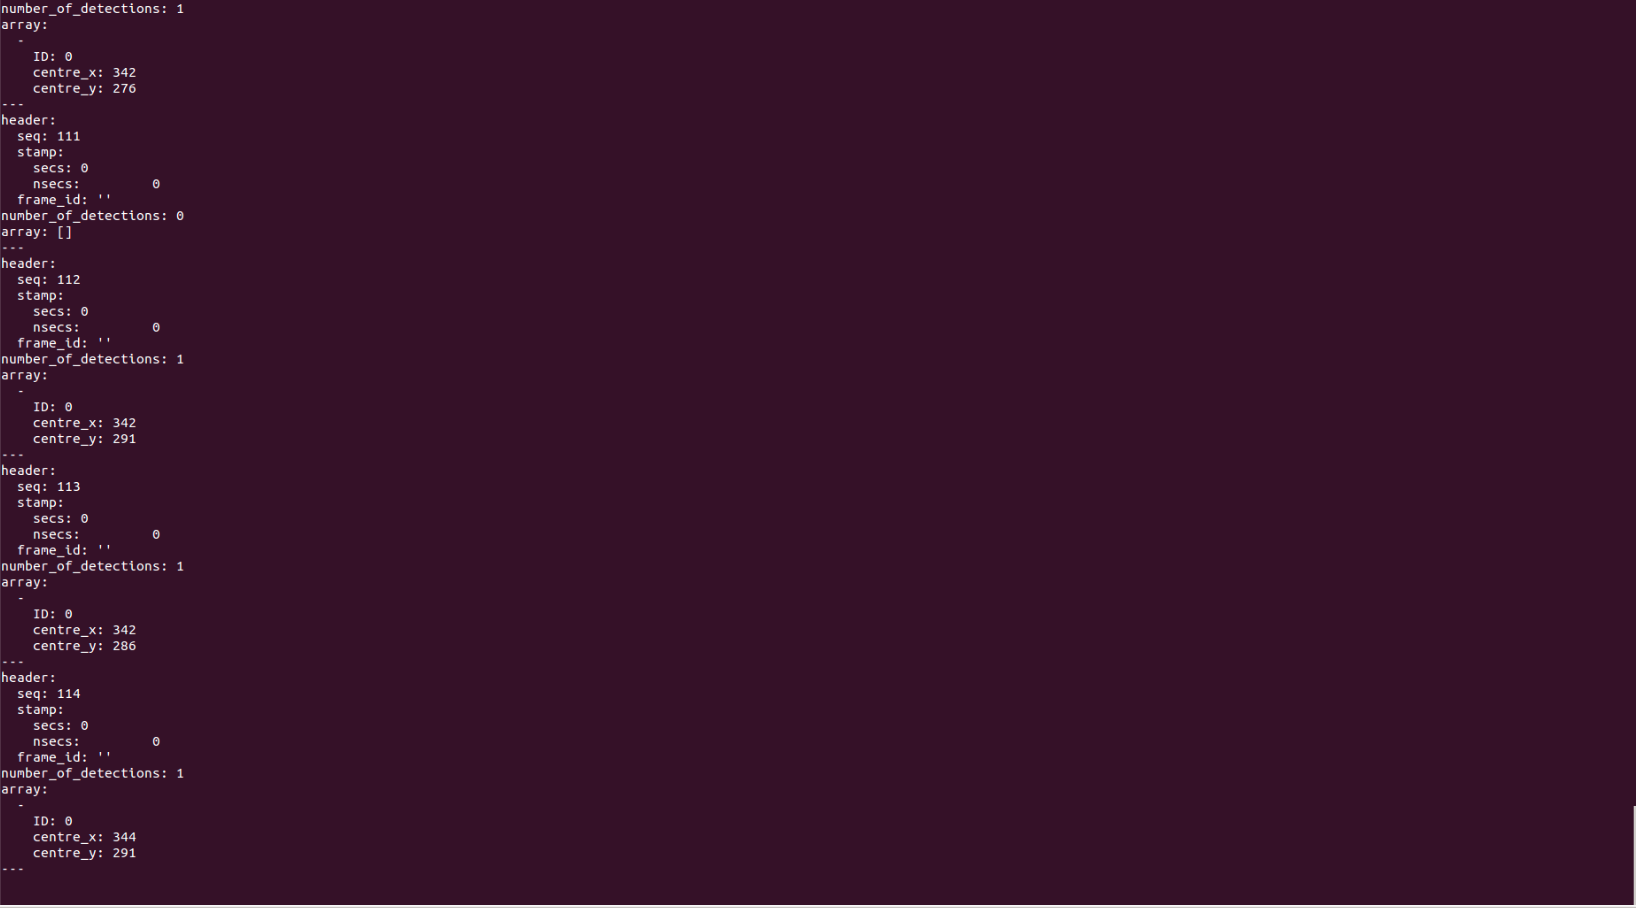
\includegraphics[width=.9\linewidth]{images/chapter3_detections_topic.png}
  \end{center}
  \caption{Detections topic output.}
  \label{fig:det_topic}
\end{figure}

